\documentclass[a4paper, 12pt]{report}

\usepackage{url}
\usepackage{graphicx}
\usepackage{amsmath}
\usepackage{eurosym}

\title{Software Engineering Group 2 (2009-2010) \\Software Design Document}
\author{Bart Maes}
\date {November 27, 2009}

\makeindex



\begin{document}

\maketitle

\thispagestyle{empty}



\begin{abstract}
This document, the Software Design Description lays down the architecture and detailed design of the Salesmen software, to be conceived in the context of the annual project for the \emph{Software Engineering} course. It took place under guidance of Prof Dirk Vermeir and assistant Yoeri De Koster during the 2009-2010 study year at the Vrije Universiteit Brussel (Brussels, Belgium).
\end{abstract}

\begin{center}
\emph{Document history:}\\
\begin{tabular}{llll}
version & date & author & description \\
\hline
v1 & 27 Nov 2009 & Bart Maes & Draft initialization \\
\end{tabular}
\end{center}

\newpage
\tableofcontents
\newpage

\section{Introduction}

\subsection{Purpose}
   This document specifies the entire software architecture and design for the Salesmen software. These design decisions directly relate to the functionalities, performances, constraints, attributes and interfaces of the system.

\subsection{Scope}
    This document describes the software architecture and design for the initial release of the Salesmen software, version 1.0. The intended audience of this document exclusively includes the designers, the developers and the testers of the software.

This SDD document mainly follows the standards of the IEEE 1016-1998 standard.

\subsection{Reference materials}
\begin{itemize}
\item IEEE Std. 1016-1998 - Software Design Descriptions
\item \url{http://tinf2.vub.ac.be/~dvermeir/courses/software_engineering/slides.pdf} [1 Nov 2009].
\end{itemize}

\subsection{Definitions and acronyms (listed alphabetically) \label{acronyms}}
\begin{tabular}{ll}
\textbf{SCMP}   & Software Configuration Management Plan \\
\textbf{SDD}    & Software Design Document \\
\textbf{SMTP}   & Single Mail Transfer Protocol \\
\textbf{SPMP}   & Software Project Management Plan \\
\textbf{SQAP}   & Software Quality Assurance Plan \\
\textbf{SRS}    & Software Requirements Specification \\
\textbf{STD}    & Software Test Document\\
\textbf{SVN}    & Subversion, a version control system\\
\textbf{QA}     & Quality Assurance\\
\end{tabular}

\pagebreak
\section{System Architecture}
\subsection{Overview}

\begin{figure}
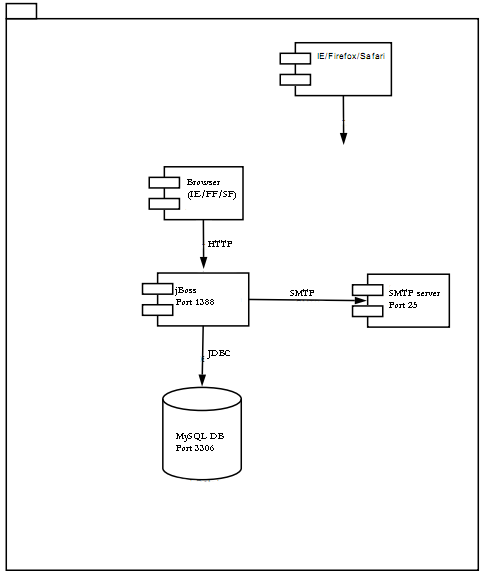
\includegraphics[scale=0.8]{../../img/archi1.png}
\caption{Salesmen Architecture}
\end{figure}

\subsection{Three-Tier Architecture}
Three-tier is a client-server architecture in which the user interface, functional process logic, computer data storage and data access are developed and maintained as independent modules, most often on separate platforms.

Apart from the usual advantages of modular software with well defined interfaces, the three-tier architecture is intended to allow any of the three tiers to be upgraded or replaced independently as requirements or technology change. For example, a change of operating system in the presentation tier would only affect the user interface code.

Typically, the user interface runs on a desktop PC or workstation and uses a standard graphical user interface, functional process logic may consist of one or more separate modules running on a workstation or application server, and an RDBMS on a database server or mainframe contains the computer data storage logic.

Three-tier architecture has the following three tiers:
\begin {itemize}
\item \textbf{Presentation tier}
This is the topmost level of the application. The presentation tier displays information related to such services as browsing merchandise, purchasing, and shopping cart contents. It communicates with other tiers by outputting results to the browser/client tier and all other tiers in the network.
\item \textbf{Application tier (Business Logic/Logic Tier)}
The logic tier is pulled out from the presentation tier and, as its own layer, it controls an application�s functionality by performing detailed processing.
\item \textbf{Data tier}
This tier consists of Database Servers. Here information is stored and retrieved. This tier keeps data neutral and independent from application servers or business logic. Giving data its own tier also improves scalability and performance. 
\end {itemize}
Benefits of using this architectural style include increased performance, flexibility, maintainability, reusability, and scalability.
\subsection{Discussion of Alternative Designs}
\textbf{MVC}
At first glance, the three tiers may seem similar to the MVC (Model View Controller) concept; however, topologically they are different. A fundamental rule in a three-tier architecture is the client tier never communicates directly with the data tier; in a three-tier model all communication must pass through the middleware tier. Conceptually the three-tier architecture is linear. However, the MVC architecture is triangular: the View sends updates to the Controller, the Controller updates the Model, and the View gets updated directly from the Model.

From a historical perspective the three-tier architecture concept emerged in the 1990s from observations of distributed systems (e.g., web applications) where the client, middleware and data tiers ran on physically separate platforms. Whereas MVC comes from the previous decade and is based on observations of applications that ran on a single graphical workstation; MVC was applied to distributed applications much later in its history.


\subsection{Survey of Technologies Used}
\subsubsection{Presentation Layer}
Java Server Pages (JSP) is a technology from Sun that allows easy development of GUIs using webbrowser clients. JSP helps in making a clear distinction of layout and code concepts, so that a developer and graphical designer can independently work on the same webpages with little interference.

\subsubsection{Business Layer}
JBoss Application Server (or JBoss AS) is a free software/open-source Java EE-based application server. Because it is Java-based, the JBoss application server operates cross-platform: usable on any operating system that Java supports. 
As part of the jBoss software, the Apache Tomcat servlet container will allow us to serve dynamically parsed webpages (JSP). 


\subsubsection{Data Layer}
Two database platforms were considered: MySQL and PostgresSQL.

Our programmers will not need to write SQL statements themselves, as these are generated with the use of the EJB3 standard and Java annotations. 
Based on Hibernate concepts, EJB3 allows for persintant objects without the need for platform dependant SQL statements and other 'dirty' constructs.


\subsection{Physical Configuration}
The software is to be installed on the Wilma server at the VUB datacenter. Wilma is accessible over the internet through web browsers and command line clients. The software relies on the availability of an SMTP server on the local LAN of the VUB, so that we do not have to include MDA (Mail Delivery Agent) functionality in the software.

\begin{figure}
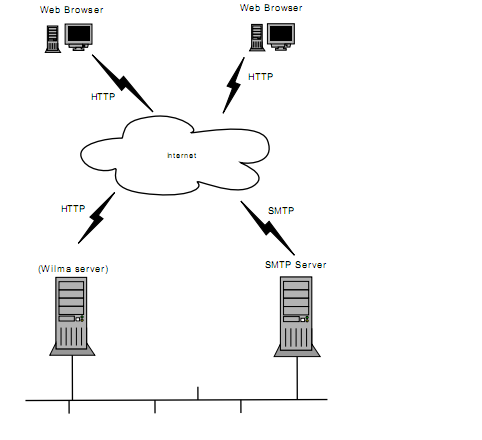
\includegraphics[scale=0.8]{../../img/infra1.png}
\caption{Salesmen infrastructure}
\end{figure}


\subsection{System Interface Description}
The web-interface is the only interface available to users of the Salesmen software. However, depending of the access-rights provided to a given user, more options may become available. Website administrators, for example, can close auctions or ban other members while 'normal' members cannot access these facilities. A more detailed description of the access-rights provided to each group of users will be provided in the SRS.
\pagebreak
\section{Component Design \label{Component Design}}
?
\section{Software Features}
[[[Hier all use cases toevoegen...]]]

% ------------------------------------------------------------------------
% Begin Use Cases
% ------------------------------------------------------------------------


% ------------------------------------------------------------------------
% End of Use Cases
% ------------------------------------------------------------------------

\pagebreak
\section{User Interface Design \label{UI Design}}
\subsection{Web pages tree}
\subsubsection{Overview}
(pagetree image)

\subsubsection{Page Description}
\begin{itemize}
\item index.jsp: welcome page of the website, invites guests to register, shows advertising, features auctions,..
\item login.jsp: allows a guest to log in. Every page will feature a login-form, login.jsp will handle the business logic (check password etc)
\item logout.jsp: destroys the current session, logs the member out
\item auctionlist.jsp: shows both an overview of subcategories and a list of auctions within this category. It features a 'filter' form that allows to shrink the current auctionlist according to provided keywords (~ search within current list). When no category is specified, the top-level category is shown.
\item auctiondetail.jsp: shows details of the given auction. When no (or an illegal) auction is specified, an error is shown. It also features bidding-facilities, show a history of bids, an interface to view pictures of the items sold and comments added by the sellers of potential buyers.
\item newauction.jsp: allows a member to add a new auction to the website. The provided form will request vital information like the auctionname, the duration of the auction, a description of the items sold, the required minimum amount for which the item will be sold and facilities to upload pictures of the given item.
\item profile.jsp: features the user control panel, to allow a member to change his personal information. It also allows a member to manage favorite sellers, the buyers assistant and followed auctions.
\item search.jsp: provides powerful search-options using keywords, tags and (multiple) categories.
\end{itemize}
\pagebreak
\subsection{User Interface}
\begin{figure}
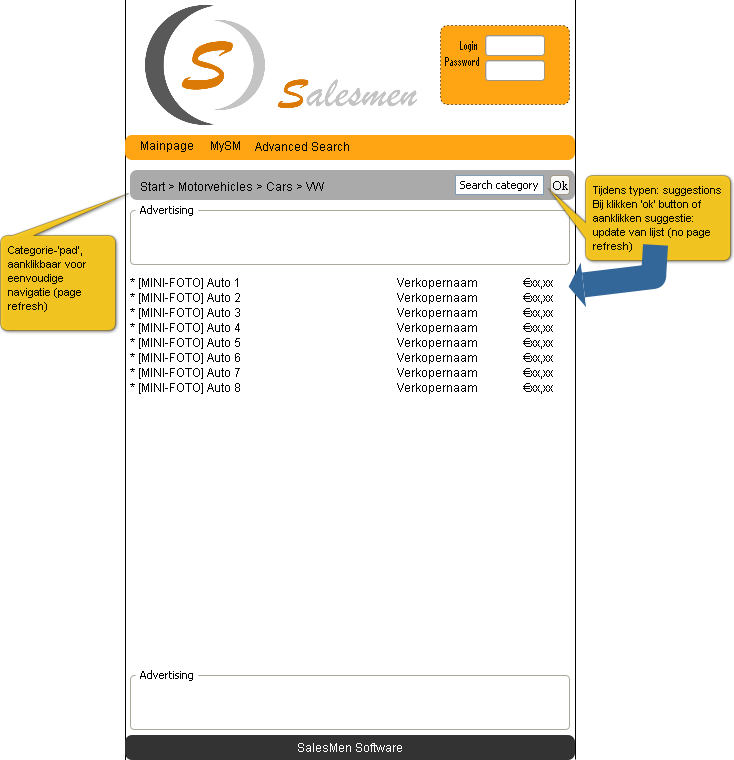
\includegraphics[width=15cm]{../../img/SM_auction_list.png}
\caption{auctionlist.jsp}
\end{figure}
\begin{figure}
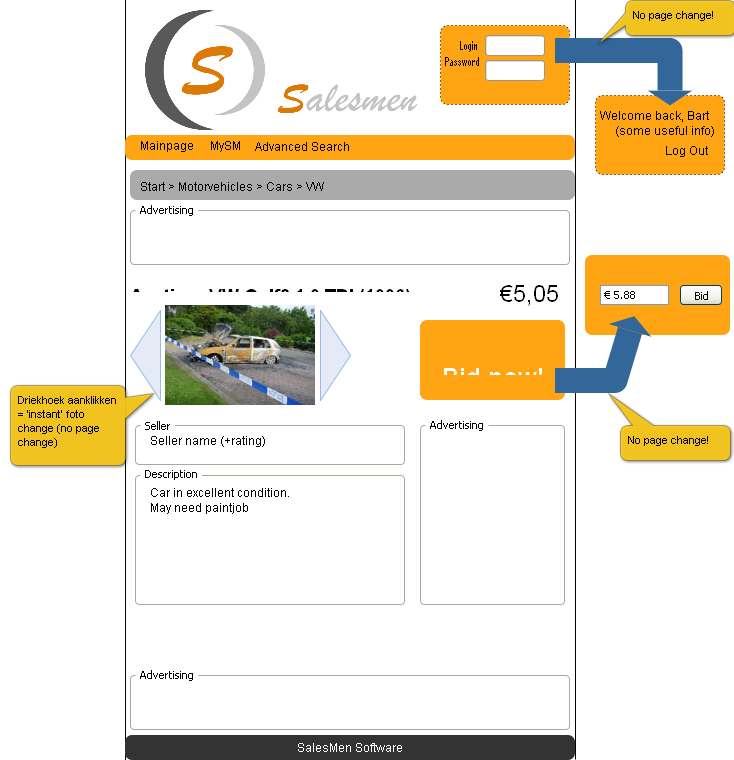
\includegraphics[width=15cm]{../../img/SM_auction_detail.png}
\caption{auctiondetail.jsp}
\end{figure}
\begin{figure}
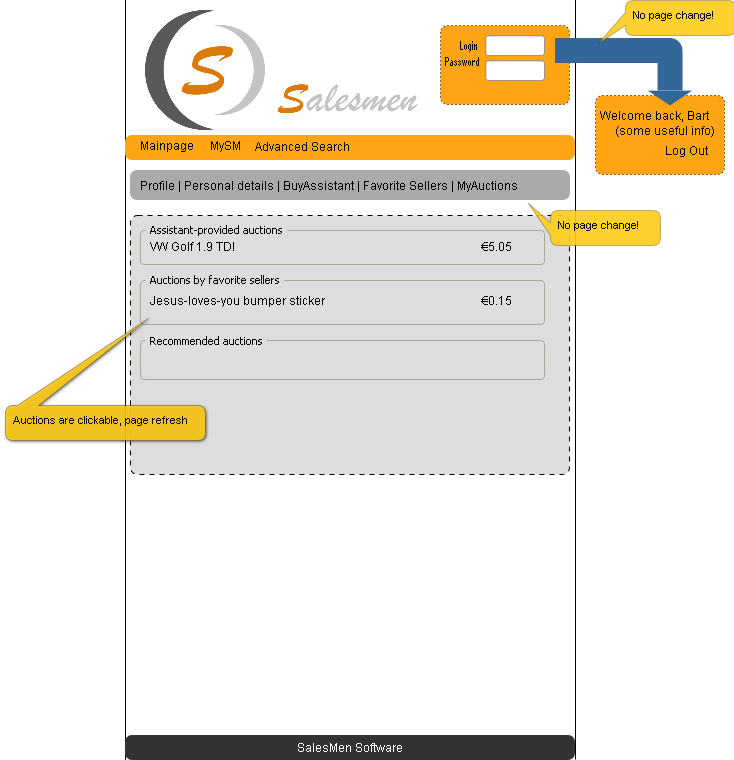
\includegraphics[width=15cm]{../../img/SM_mySM_auctions.png}
\caption{profile.jsp - auctions}
\end{figure}
\begin{figure}
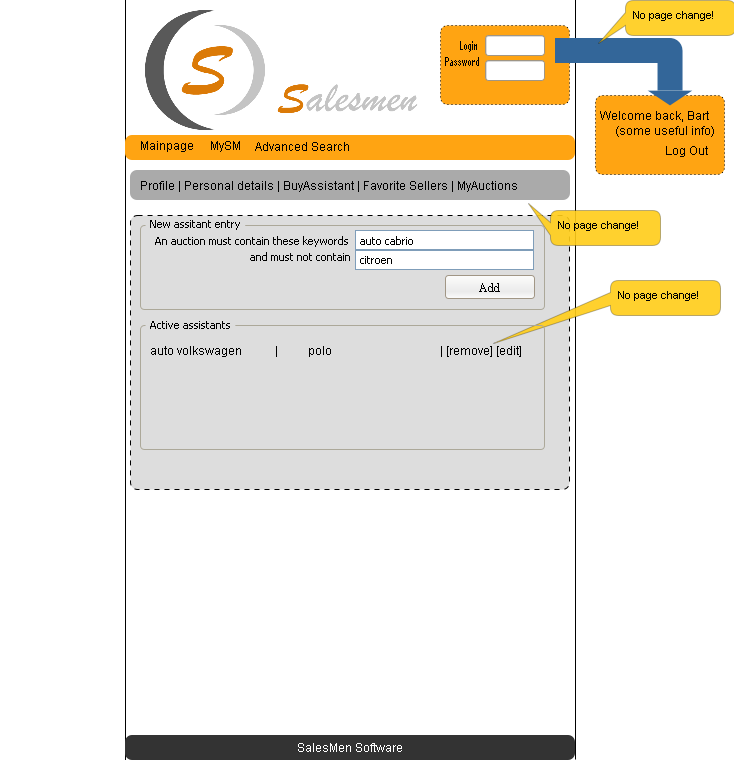
\includegraphics[width=15cm]{../../img/SM_mySM_buy_assistant.png}
\caption{profile.jsp - buyers assistant}
\end{figure}
\begin{figure}
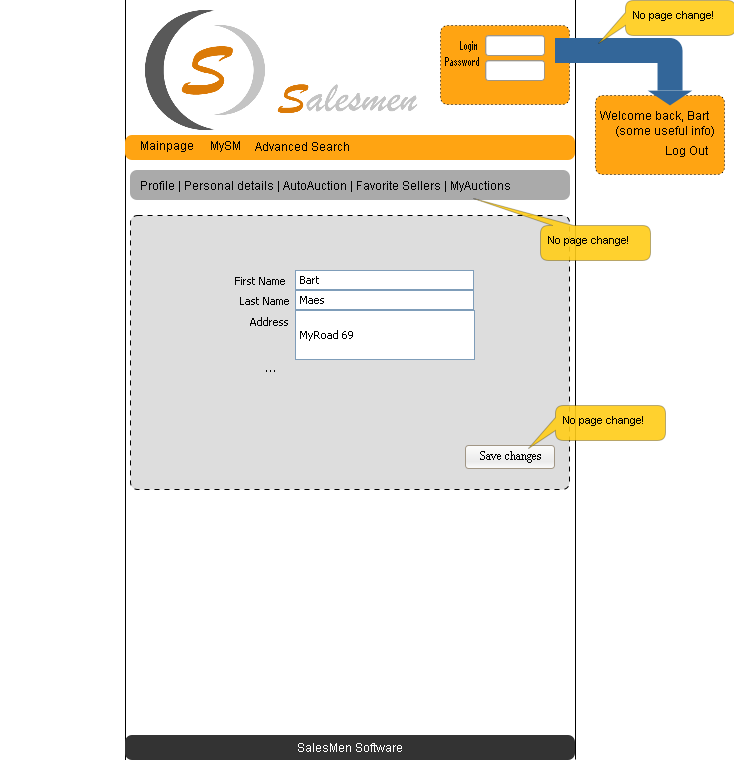
\includegraphics[width=15cm]{../../img/SM_mySM_personal.png}
\caption{profile.jsp - personal information}
\end{figure}
\begin{figure}
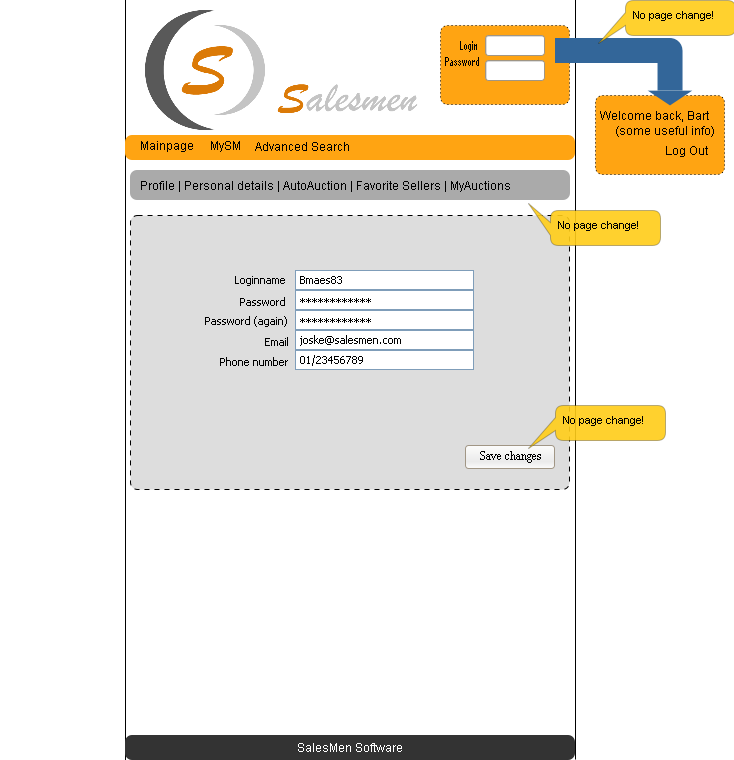
\includegraphics[width=15cm]{../../img/SM_mySM_profile.png}
\caption{profile.jsp - website information}
\end{figure}

\section{Database Design}
\begin{figure}
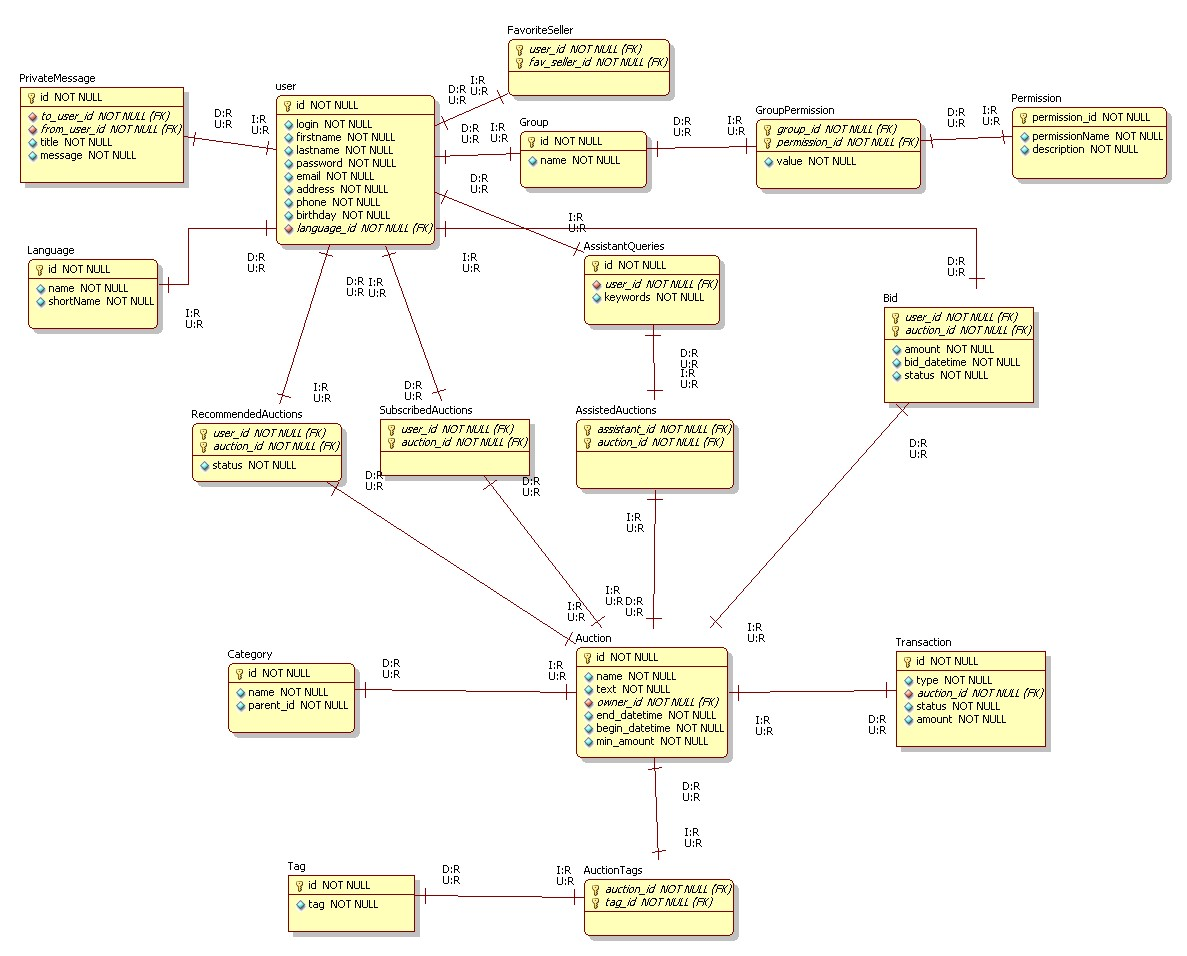
\includegraphics[scale=0.5,angle=90]{../../img/erd1.jpg}
\caption{Salesmen database layout}
\end{figure}

\section{Additional Material \label{Additional}}
\section{Requirements Traceability Matrix}

\end{document}
